\section{TP3: Push Push}
\subsection{Objectif}
Dans cette manipulation nous allons voir comment faire intéragir des modules d'entrées avec des modules de sortie pour par exemple, allumer une LED par appuis sur un bouton, afficher le une valeur correspondant à un bouton sur un matrice ou encore faire intéragie une matrice de led avec un joystick.
\
subsection{Matériel}a
\begin{itemize}
	\item Un ordinateur
	\item Un arduino Uno R3
	\item Un boutton poussoir
	\item Des resistance de 10K$\Omega$
	\item Une led
	\item Une matrice de boutons
	\item Un afficheur LCD
	\item Un Joystick
	\item Une matrice de LED
\end{itemize}


\subsection{LED et boutton}

\lstinputlisting[language=C]{Code/TP3/TP3.1/TP3.1.ino}
\begin{figure}[H]
	\centering
	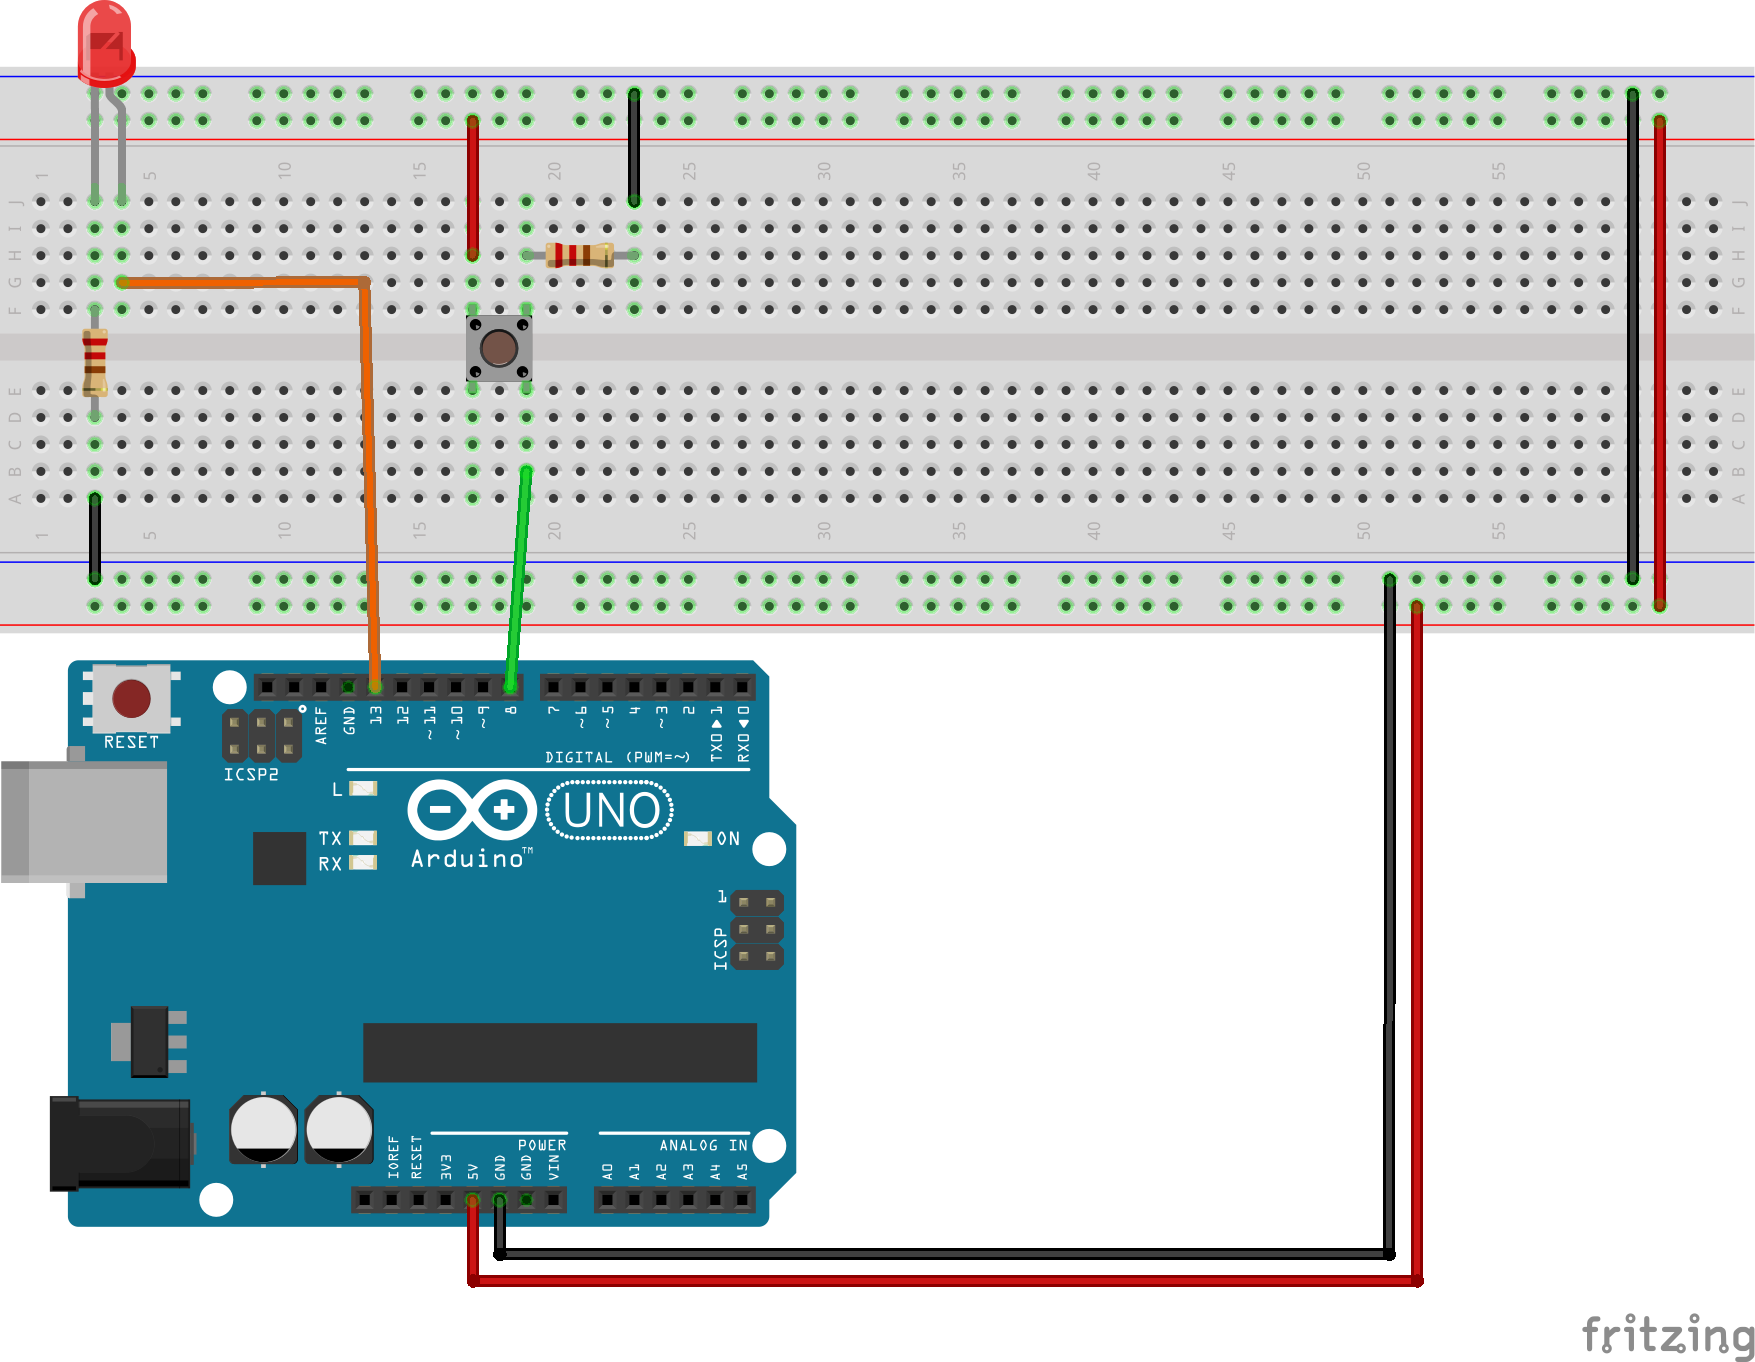
\includegraphics[height=6cm]{img/TP3-1.png}
	\caption{\label{TP3.1}LED et boutton}
\end{figure}
%TODO Button

\subsection{Debounce}

\lstinputlisting[language=C]{Code/TP3/TP3.2/TP3.2.ino}
\begin{figure}[H]
	\centering
	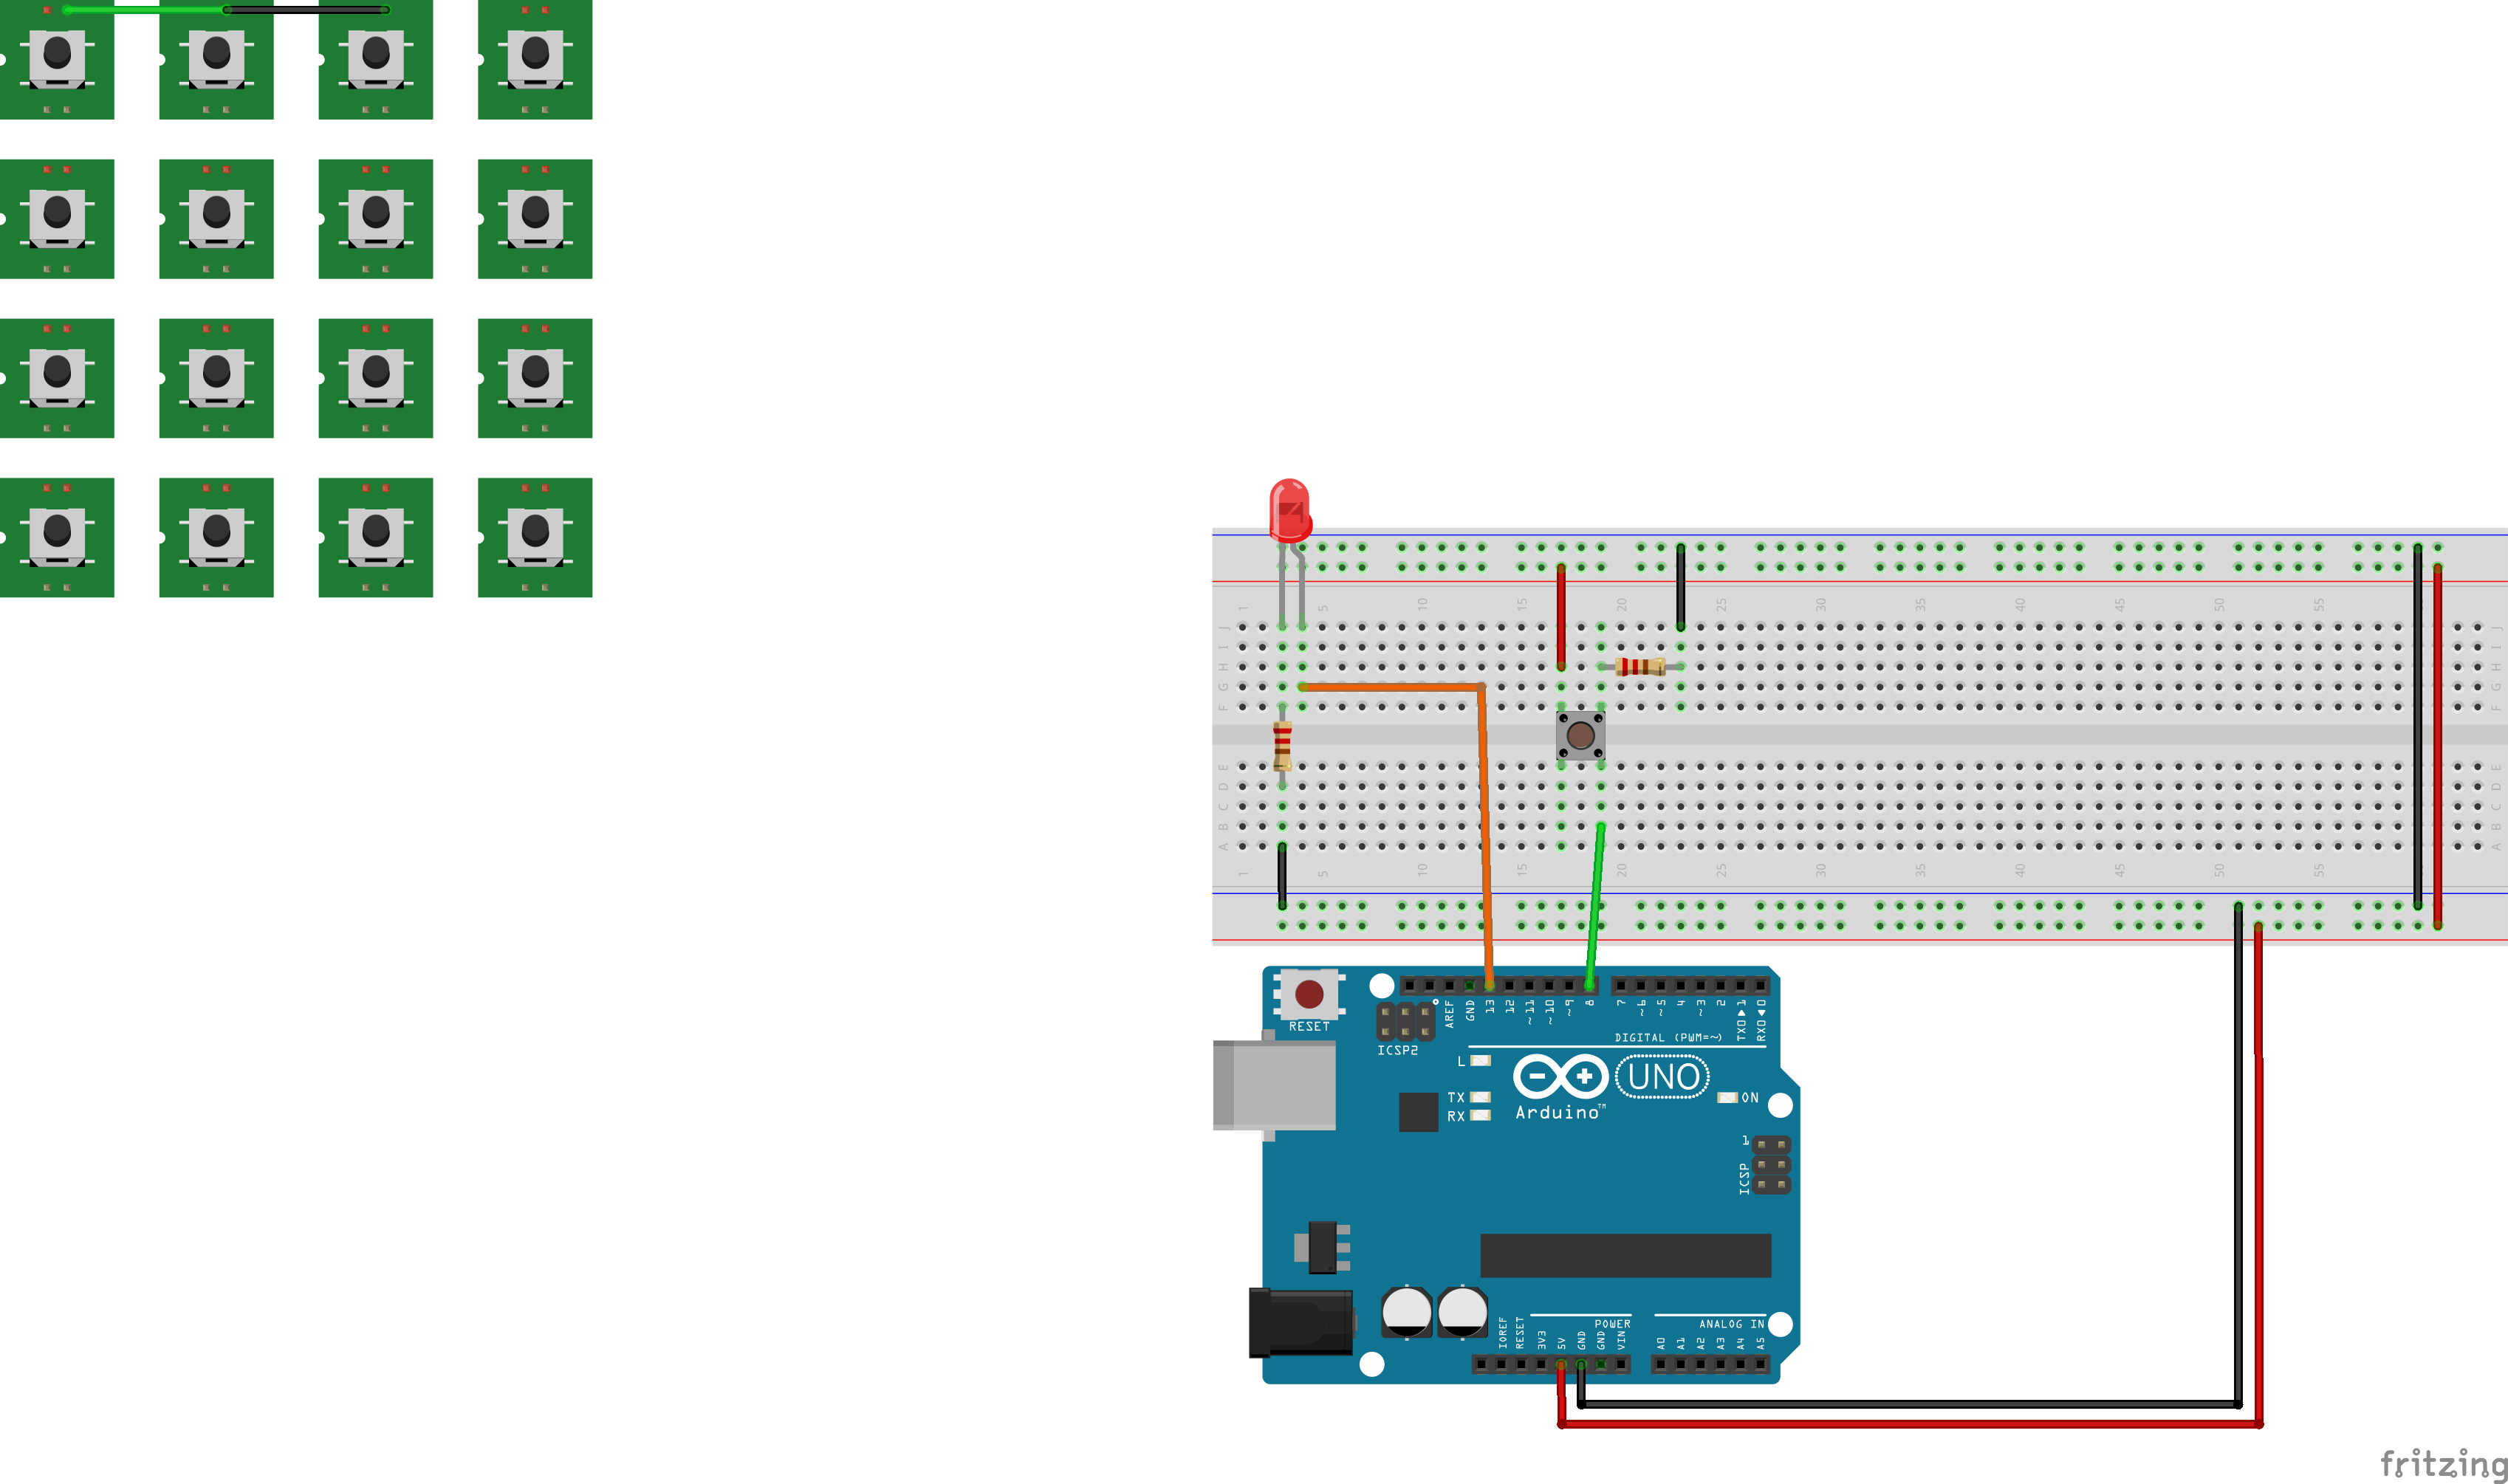
\includegraphics[height=6cm]{img/TP3-2.png}
	\caption{\label{TP3.2}Debounce}
\end{figure}
\subsection{Matrice de bouttons}

\lstinputlisting[language=C]{Code/TP3/TP3.3/TP3.3.ino}
\begin{figure}[H]
	\centering
	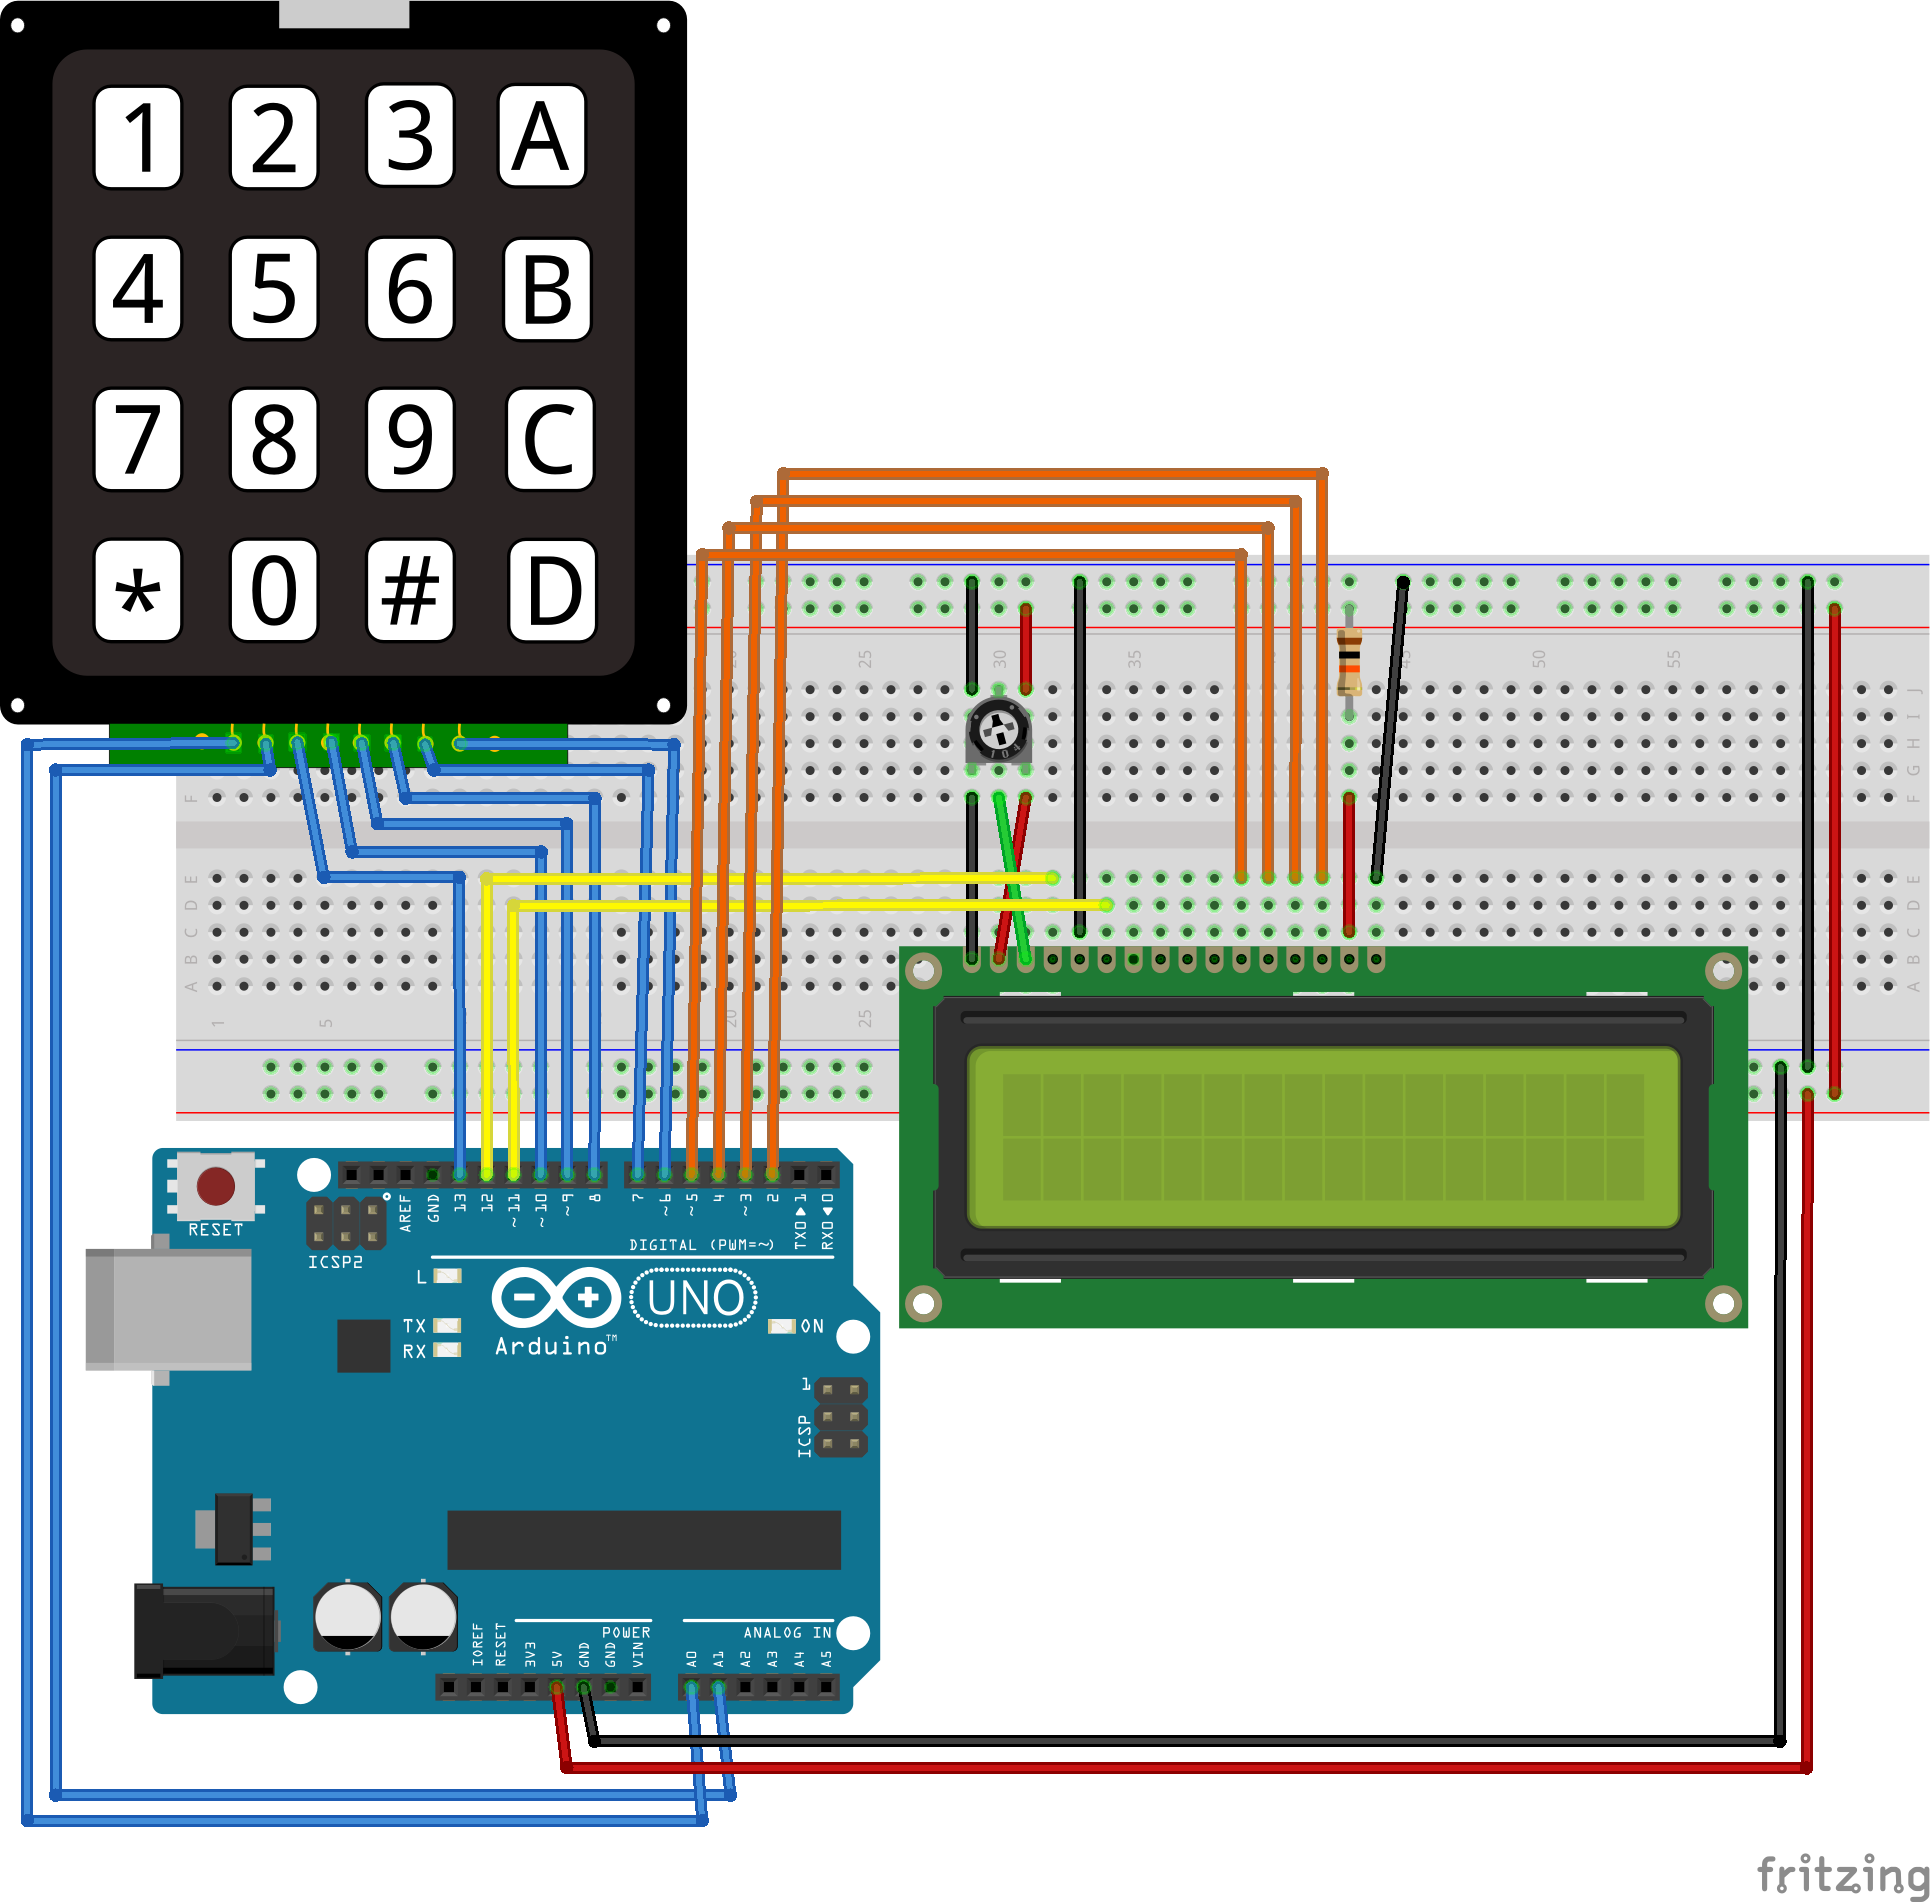
\includegraphics[height=6cm]{img/TP3-3.png}
	\caption{\label{TP3.3}Matrice de bouttons}
\end{figure}

% \subsection{Joystick et matrice de LED}

% \lstinputlisting[language=C]{Code/TP3/TP3.4/TP3.4.ino}
% \begin{figure}[H]
% 	\centering
% 	\includegraphics[height=6cm]{img/TP3-4.png}
% 	\caption{\label{TP3.4}Joystick et matrice de LED}
% \end{figure}
%%TODO Matrice button
